\documentclass[11pt,a4paper]{article}
\usepackage[utf8]{inputenc}
\usepackage[T1]{fontenc}
\usepackage{mathpazo}
\usepackage[margin=2.5cm]{geometry}
\usepackage{amsmath,amssymb}
\usepackage{booktabs,array,xcolor,graphicx,float}
\usepackage[colorlinks=true,linkcolor=blue!45!black,urlcolor=blue!45!black]{hyperref}
\setlength{\parskip}{0.5em}\setlength{\parindent}{0pt}
\setlength{\emergencystretch}{2em}
\renewcommand{\arraystretch}{1.25}
\newcolumntype{L}[1]{>{\raggedright\arraybackslash}p{#1}}
\newcommand{\code}[1]{\texttt{#1}}
\newcommand{\tauv}{\tau}
\title{How to read the results of \texttt{pde-factor-fit}\\[2pt]\large The returned numbers, the returned distributions, the p-values and the direction images}
\author{Flavio Pricoco}
\date{}
\begin{document}
\maketitle
\begin{abstract}\noindent
This guide says what every output of the algorithm \emph{means} and how to read it; it does not explain how the algorithm computes it (see \code{paper/structure\_B.pdf} for that). Everything is illustrated on one real run: \code{python benchmarks/final\_report.py --case transport\_plus\_diffusion --noise 0.05}. The data were generated by $(\partial_t+\partial_x)(\partial_t-0.3\,\partial_x^2)u=0$ (a transport factor and a diffusion factor) on a $64\times128$ grid with 5\% noise, so the answer is known and you can see how far off the output is.
\end{abstract}

\section{Where the results come from}
A run produces a result object \code{res} (from \code{run\_loop}) and, with \code{benchmarks/final\_report.py}, a folder with
\code{report.md} (everything in readable form), \code{report.json} (the same, machine readable) and five images (Section~\ref{sec:img}). In Python: \code{res.label}, \code{res.equation()}, \code{res.summary()}.

\textbf{Conventions.} $\tau$ stands for $\partial/\partial t$ and $\xi$ for $\partial/\partial x$; $\kappa$ is the spatial wavenumber (a mode is $e^{\lambda t+i\kappa x}$). Each factor is written \emph{monic in $\tau$}, so its $\tau$-coefficient is exactly 1. The equation is the \emph{product} of the factors applied to $u$: \code{(tau + xi) * (tau - 0.3 xi**2) u = 0} means $(\partial_t+\partial_x)(\partial_t-0.3\partial_x^2)u=0$.

\section{The answer in one line: label and equation}
\begin{center}\small
\begin{tabular}{L{4.0cm}L{10.0cm}}\toprule
\textbf{field} & \textbf{how to read it}\\\midrule
\code{label} & The verdict. \textbf{FIT-COMPATIBLE}: the data are consistent with the printed product of factors (this is \emph{not} a claim that the law is identified; it only says the data do not contradict it). \textbf{MISFIT}: no structure within the search bounds explains the data. \textbf{ID-KER}: a fit exists but at least one factor is not fully supported by the data (too few modes, or too few branches at one wavenumber), so only the \emph{kernel} of that factor, not its full form, is determined; the note says why. \textbf{UNDECIDED}: the data cannot decide (for example a repeated factor is possible, or the law leaves structure in the data).\\
\code{equation()} & The product of the \emph{pruned} factors: every term whose 90\% interval (real and imaginary part) contains 0 is removed, because the posterior does not distinguish it from 0. Example run: $(\tau+0.999\,\xi+0.0082)(\tau-0.2859\,\xi^2)$. Both factors are recovered separately; the small $0.0082$ term survives because its interval $[0.0021,0.0109]$ excludes 0, although the true value is 0: a term that is ``statistically nonzero'' can still be noise-sized, so judge the \emph{size} of a term, not only its interval.\\
\code{note} & Free text: why this structure was chosen, or why a claim was withdrawn. Read it whenever the label is not FIT-COMPATIBLE.\\
\code{bounds} $(m,d_x)$ & The class that was searched: factors of $\tau$-degree up to $m$ and $\xi$-degree up to $d_x$. $(3,4)$ in the example. If the label is MISFIT, the law may lie outside these bounds.\\
\code{regrouped} & \code{True} if all posterior samples were re-fitted at the chosen structure (normal).\\\bottomrule
\end{tabular}
\end{center}

\section{Factors: one block per factor}
\begin{center}\small
\begin{tabular}{L{4.0cm}L{10.0cm}}\toprule
\textbf{field} & \textbf{how to read it}\\\midrule
\code{sympy} & The factor, e.g. \code{tau + 0.999 xi + 0.0082}.\\
\code{W} & The factor's \emph{share of the field}: the weights of all factors sum to 1. Example: 0.759 (transport) and 0.241 (diffusion). It says how much of the observed signal lives in that factor, not how important the factor is for the physics.\\
\code{status} & Free text. ``clean (component alone: $k=1$, label FIT-COMPATIBLE)'' means: when the part of the data belonging to this factor is analysed on its own, it is again a single factor and fits. Any other text is a caveat; read it literally.\\
\code{kappa\_support} & The wavenumbers $\kappa$ at which this factor's modes were actually seen. Example: $\{1,2,3,4\}$ for transport and $\{1,2,3\}$ for diffusion (the faster-decaying diffusion modes at $\kappa=4$ fell below the noise). A short support means the factor is determined from few points.\\
\code{coef}: \code{median}, \code{q05}, \code{q95} & One row per term $\tau^a\xi^b$: posterior median and 90\% interval (5\%--95\% quantiles); complex numbers are shown as real and imaginary part. The leading $\tau$ term is exactly 1 with zero-width interval (monic). Example, diffusion term $\xi^2$: median $-0.2859$, interval $[-0.324,-0.279]$ (truth $-0.3$). A narrow interval means a well-determined coefficient \emph{given the chosen structure}; it does not include the risk that the structure itself is wrong (that is the job of $P(k)$ and the tests below).\\
\code{fit.n\_modes} & Number of kernel modes of this factor used in the component fit.\\
\code{fit.energy\_}\code{explained\_alone} & Fraction of the energy of the data that this factor's kernel modes alone reproduce ($1-\text{relative residual}^2$): 97.7\% for transport, 70.7\% for diffusion. They do \emph{not} add to 100\%: the two descriptions overlap and the remainder is explained only by the two factors together.\\
\code{fit.weight\_}\code{from\_u\_j} & Share of the norm of the fitted component $u_j$ (the part of the field attributed to factor $j$); should be close to $W$ (0.768 vs 0.759 here). A large gap between the two is a warning.\\\bottomrule
\end{tabular}
\end{center}

\section{The model: structure, evidence, levels}
\begin{center}\small
\begin{tabular}{L{4.0cm}L{10.0cm}}\toprule
\textbf{field} & \textbf{how to read it}\\\midrule
\code{P(k)} & Posterior probability of the number of factors $k$ (here $k=2$ with probability 1). A probability from model comparison, \textbf{not} a p-value. \code{p\_k\_DP} and \code{p\_k\_finite\_BIC} are the same question under two models (Dirichlet-process mixture, and a finite model compared by BIC); if they disagree, the number of factors is not settled.\\
\code{structures} & Posterior over the candidate \emph{shapes} of the factor set, e.g.\ \code{((1,1),(1,2))} = one factor of $(\tau\text{-degree},\xi\text{-degree})=(1,1)$ and one of $(1,2)$. Next to each: the \emph{log evidence} (marginal likelihood of the data under that structure, here $-503.7$). Only differences of log evidence between structures mean something: a gap of 3 or more is a clear preference.\\
\code{core\_labels} & Fraction of posterior samples that received each label before pooling.\\
\code{dropped} & Factors removed as redundant by the split evidence.\\
\code{history} (one row per level) & \code{bounds}: the class tried; \code{p\_fit}: posterior mass on FIT-COMPATIBLE at that class; \code{heldout}: mean and standard error of the capped squared standardized residual $z^2$ of modes held out of the fit (lower is better, about 1 is what noise alone gives; this is a score, not a p-value); \code{accepted}: whether the loop moved to this class. Several rows mean the loop enlarged the class because the smaller one was not enough.\\\bottomrule
\end{tabular}
\end{center}

\section{Distributions: what ``returned distribution'' means}\label{sec:dist}
Whenever a quantity is uncertain, the algorithm returns not one number but a \emph{distribution over posterior samples} (the plausible fields consistent with the data, each with weight $\pi_s$). It is always summarised as \textbf{q05 / q50 / q95} (5\%, median, 95\% quantile, so q05--q95 is a 90\% interval) and the \textbf{mean}. Read the interval width first: a narrow interval means the samples agree, a wide one that the answer depends on which plausible field you believe. With few samples (3 in the example) the distribution is coarse: the histograms in Figure~\ref{fig:dist} show three bars, one per sample, each of weight $1/3$.

\begin{center}\small
\begin{tabular}{L{4.0cm}L{10.0cm}}\toprule
\textbf{quantity} & \textbf{how to read it}\\\midrule
$k_\mathrm{eff}$, $k_\mathrm{det}$ & $k_\mathrm{eff}=\exp(-\sum_jW_j\ln W_j)$ is the ``effective number of factors'' from the weights: 2 equal factors give 2, one dominant and one faint factor give a value close to 1. Example: $1.738$ for $W=(0.759,0.241)$. $k_\mathrm{det}=\lceil k_\mathrm{eff}\rceil=2$ is the integer used for comparison. Its per-sample q05/q50/q95 ($1.711/1.739/1.762$) show how stable it is across samples.\\
\code{W\_track} / \code{track\_sympy} & The weights and symbols of the \emph{tracks}: the clusters of factors found across all samples. \textbf{Track order is not factor order} (here track 0 is diffusion, factor 0 is transport); always match by the printed formula.\\
\code{theta\_bar}, \code{theta\_sd} & Mean and standard deviation of the coefficient vector of each track over the samples (real parts, then imaginary parts, of the coefficients of $\tau^a\xi^b$).\\
$c_F$ (q05/50/95) & Cosine of the Friedrichs angle between the solution spaces (kernels) of two factors: 0 means the two kinds of solutions are well separated, 1 means they cannot be told apart. Example: $0.826/0.838/0.840$ (angle about $0.58$ rad).\\
$\gamma$ & $\gamma=1-c_F$ for two factors, more generally the smallest eigenvalue of the block Gram matrix of the kernel bases. The error on each factor's component is amplified by $\gamma^{-1/2}$ (here $\gamma_N=0.166$, amplification $2.46$): the closer $\gamma$ is to 0, the less reliably the data can split the field into its factors.\\
$\rho$ ($E_\mathrm{int}$) & Size of the interaction term, relative to the change of the solution over the window, $\|E_\mathrm{int}\|/\|u(T)-u_0\|$: small means the factors act almost independently; larger means that treating them separately would miss a visible part of the evolution. Example median $0.059$. The report says ``computed'' or ``not computed by core v2''; ignore the number in the second case.\\
$P(\text{split})$, $P(\text{include}_j)$, $w_j$ & From the Bayesian split layer: $P(\text{split})$ is the posterior probability that the field really is a sum of \emph{separate} factor components (here 1.0); $P(\text{include}_j)$ that factor $j$ is really present; $w_j$ the mean weight of factor $j$ with its 90\% interval ($0.772\,[0.770,0.773]$ and $0.228\,[0.227,0.230]$). \code{p\_subset} lists the probability of each subset of factors; here the full set $(0,1)$ has 1.0. The split layer's own $c_F$/$\gamma$ are computed on its own basis and may differ from the headline $\gamma_N$ above; quote the block-Gram $\gamma_N$.\\\bottomrule
\end{tabular}
\end{center}

\begin{figure}[H]\centering
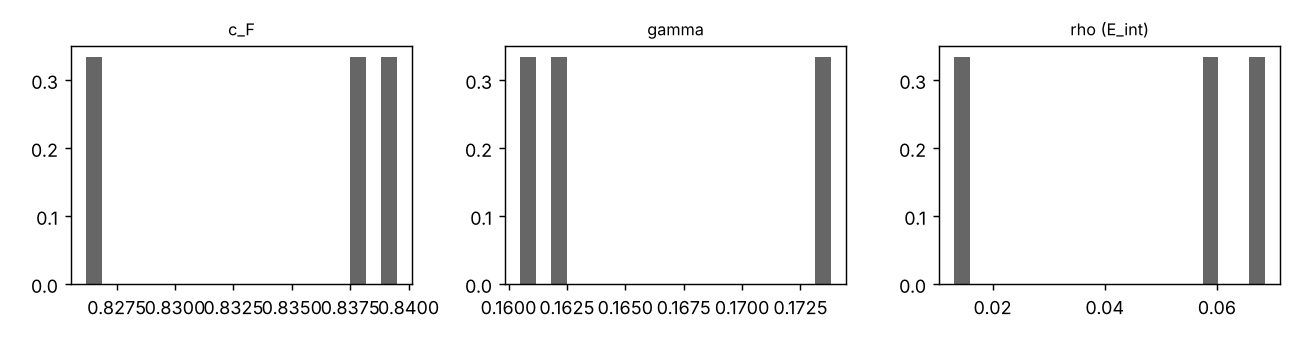
\includegraphics[width=0.95\textwidth]{figures/rr_distributions.png}
\caption{\code{distributions.png}: weighted histograms over the posterior samples of $c_F$, $\gamma$ and $\rho$. Each bar is one sample (three samples, weight $1/3$ each). Tight bars: the quantity is stable. Note the different $x$-axes: $c_F$ varies only in the second decimal.}\label{fig:dist}
\end{figure}

\section{Which p-value, of which test?}
Three different things are printed and they must not be confused.

\textbf{(a) Posterior probabilities} ($P(k)$, \code{p\_fit}, $P(\text{split})$, $P(\text{include})$, the structure posterior): outputs of model comparison, between 0 and 1, \emph{not} p-values. A value of 1.000 means ``within the models considered, this one wins decisively''.

\textbf{(b) Goodness-of-fit p-values, always reported as $\log_{10}p$} (so $-3$ means $p=10^{-3}$). All of them are \emph{$\chi^2$ tests with known noise level $\sigma$}, with the same null hypothesis and the same direction:
\begin{center}\small
\begin{tabular}{L{4.2cm}L{9.8cm}}\toprule
\textbf{null hypothesis $H_0$} & the reported law holds exactly, and what is left in the data after removing it is white Gaussian noise of standard deviation $\sigma$.\\
\textbf{alternative} & the law leaves structure in the data (it is wrong, incomplete, or the class is too small).\\
\textbf{small $p$ means} & reject $H_0$: structure is left over, the law is \emph{not claimed}.\\
\textbf{large $p$ means} & only that the test did not find a misfit. It does \textbf{not} prove the law: that is why the label is FIT-COMPATIBLE and never ``identified''.\\\bottomrule
\end{tabular}
\end{center}
The three tests differ only in what they fit the residual with:
\begin{itemize}
\item \textbf{Predictive omnibus test (V0.1).} Per Fourier bin $\kappa$, the time series of the data is fitted by least squares with the exponentials $e^{\lambda t}$ that the reported factors allow at that $\kappa$; the squared residuals, divided by the noise variance, give a $\chi^2$ statistic for that bin. The bin statistics and their degrees of freedom are summed (the \emph{omnibus} $\chi^2$) and one survival-function $p$ is computed. Used on the weightiest sample, for white noise.
\item \textbf{Smooth-residual test (T96).} After the law is fitted, the residual in each excited bin is projected on a smooth basis (Legendre polynomials in $t$); if smooth structure remains, it is not noise. Two exact tests are run, the \emph{worst bin} (Bonferroni-corrected for the number of bins, which catches an early-time misfit in one bin) and the \emph{omnibus} (which catches a misfit spread thinly over many bins), and combined by a further Bonferroni factor 2. Applied to the final FIT-COMPATIBLE law on grid data.
\item \textbf{Raw-observation test (T88/T101).} For scattered observations: least squares of the raw observations on the kernel basis of the reported law, $\chi^2$ with known $\sigma$, truncated at a maximum $|\kappa|$.
\end{itemize}
\textbf{Decision level.} A fixed level $\log_{10}p<-3$ (constant \code{PRED\_LOGP}, a test level, not a tuned parameter) withdraws the claim: the label becomes MISFIT (raw-observation test) or UNDECIDED (smooth-residual test) and the note quotes the $\log_{10}p$, the worst bin and the $\chi^2$ with its degrees of freedom. The same level also triggers the loop to try a larger class before giving up.

\textbf{How to use them in practice.} (i) These tests assume the $\sigma$ you gave: if $\sigma$ is too small the tests reject good laws, if too large they lose power. (ii) Several tests are run, so a single borderline $\log_{10}p$ near $-3$ should be read as ``look at the note'', not as a verdict. (iii) A very negative value ($-10$ or lower) in a bin is the signature of a missing factor or a too-small class.

\textbf{(c) Held-out score.} The mean and standard error of capped $z^2$ on held-out modes, in the \code{history}; a score to compare two classes (the larger class is accepted only if it is not worse by more than two standard errors), not a p-value.

\section{Reading the images}\label{sec:img}
Run \code{benchmarks/final\_report.py} and open the five \code{.png} files. All of them show the same objects in different views: the \emph{factors}, as sets of modes.

\subsection{Why ``directions'': what a pixel is}
A factor is a polynomial $Q(\tau,\xi)$ (its symbol). A mode $e^{\lambda t+i\kappa x}$ is annihilated by the factor exactly when $Q(\lambda,i\kappa)=0$. So the natural picture is the \emph{frequency plane}: the horizontal axis is $\kappa$, the vertical axis is $\lambda=\mathrm{Re}\,\lambda+i\,\mathrm{Im}\,\lambda$. Each pixel is one candidate mode; neighbouring pixels are neighbouring Fourier modes. The colour is $\log_{10}|Q(\lambda,i\kappa)|$: \textbf{dark means $|Q|\approx0$, i.e.\ the modes that factor can carry} (its kernel, the \emph{dispersion variety}); bright means the factor kills nothing there. Reading a factor is reading the dark curve.

Because $\lambda$ is complex, each factor gets \emph{two} images: the \textbf{oscillation} slice (top row: $\kappa$ against $\mathrm{Im}\,\lambda$) and the \textbf{damping} slice (bottom row: $\kappa$ against $\mathrm{Re}\,\lambda$). To reduce three coordinates $(\kappa,\mathrm{Re}\,\lambda,\mathrm{Im}\,\lambda)$ to two, each pixel shows the \emph{minimum} of $\log_{10}|Q|$ over the third coordinate, so a dark curve means ``there is a mode on this curve for some value of the hidden coordinate''.

\begin{figure}[H]\centering
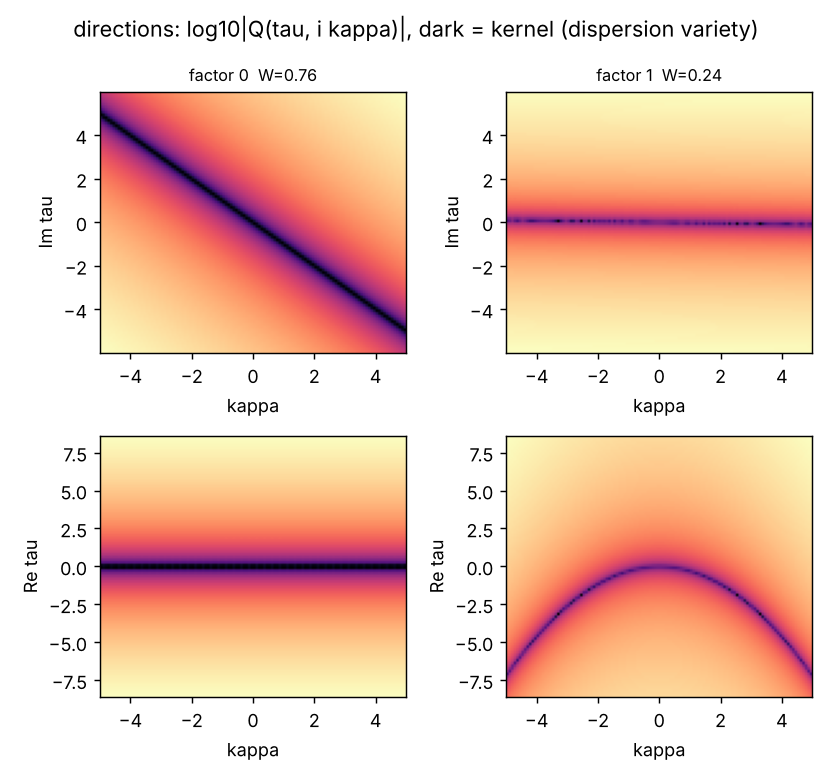
\includegraphics[width=0.78\textwidth]{figures/rr_directions.png}
\caption{\code{directions.png} for the example. Left column, factor 0 (weight 0.76), $\tau+0.999\,\xi$: top, a straight line $\mathrm{Im}\,\lambda=-\kappa$ (a wave moving at constant speed: each wavenumber oscillates at a frequency proportional to it); bottom, a flat line at $\mathrm{Re}\,\lambda=0$ (no damping). That pair is \emph{transport}. Right column, factor 1 (weight 0.24), $\tau-0.286\,\xi^2$: top, a line at $\mathrm{Im}\,\lambda=0$ (no oscillation); bottom, a parabola $\mathrm{Re}\,\lambda=-0.29\,\kappa^2$ (high wavenumbers decay fast). That pair is \emph{diffusion}.}
\end{figure}

\textbf{Quick dictionary.} Tilted line in the oscillation row + flat line at 0 in the damping row = transport/wave-like propagation. Flat line at 0 in the oscillation row + curve bending downwards in the damping row = diffusion (the steeper the parabola, the larger the diffusion constant). Curves in both rows = damped waves. A factor of higher degree shows several dark curves (one per branch of its roots). A \emph{blurry or broken} dark line means the coefficients are poorly determined; a dark line that bends upward (growth, $\mathrm{Re}\,\lambda>0$) means an unstable law and should be checked against the data.

\subsection{\texttt{directions\_uncertainty.png}: how sure are the directions}
\begin{figure}[H]\centering
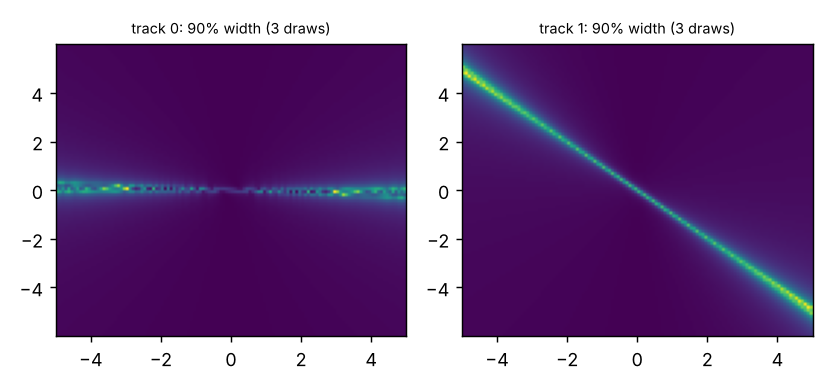
\includegraphics[width=0.7\textwidth]{figures/rr_directions_uncertainty.png}
\caption{Width of the 90\% band (95th minus 5th percentile) of the oscillation image over posterior draws of each track. Dark: the draws agree. Bright: the draws disagree at that pixel. The brightness sits along the dark curve of the factor (this is where the curve could be shifted slightly), so the brightness of that line is the uncertainty of the coefficients. Here track 1 (the transport line) is slightly uncertain in its slope; track 0 (diffusion, nearly horizontal) shows speckle because its curve is almost degenerate in this slice. \emph{Remember track order is not factor order} (Section~\ref{sec:dist}). With only 3 draws the picture is rough; with more samples it smooths.}
\end{figure}

\subsection{\texttt{operator\_space.png}: how different are the factors from each other and from the posterior draws}
\begin{figure}[H]\centering
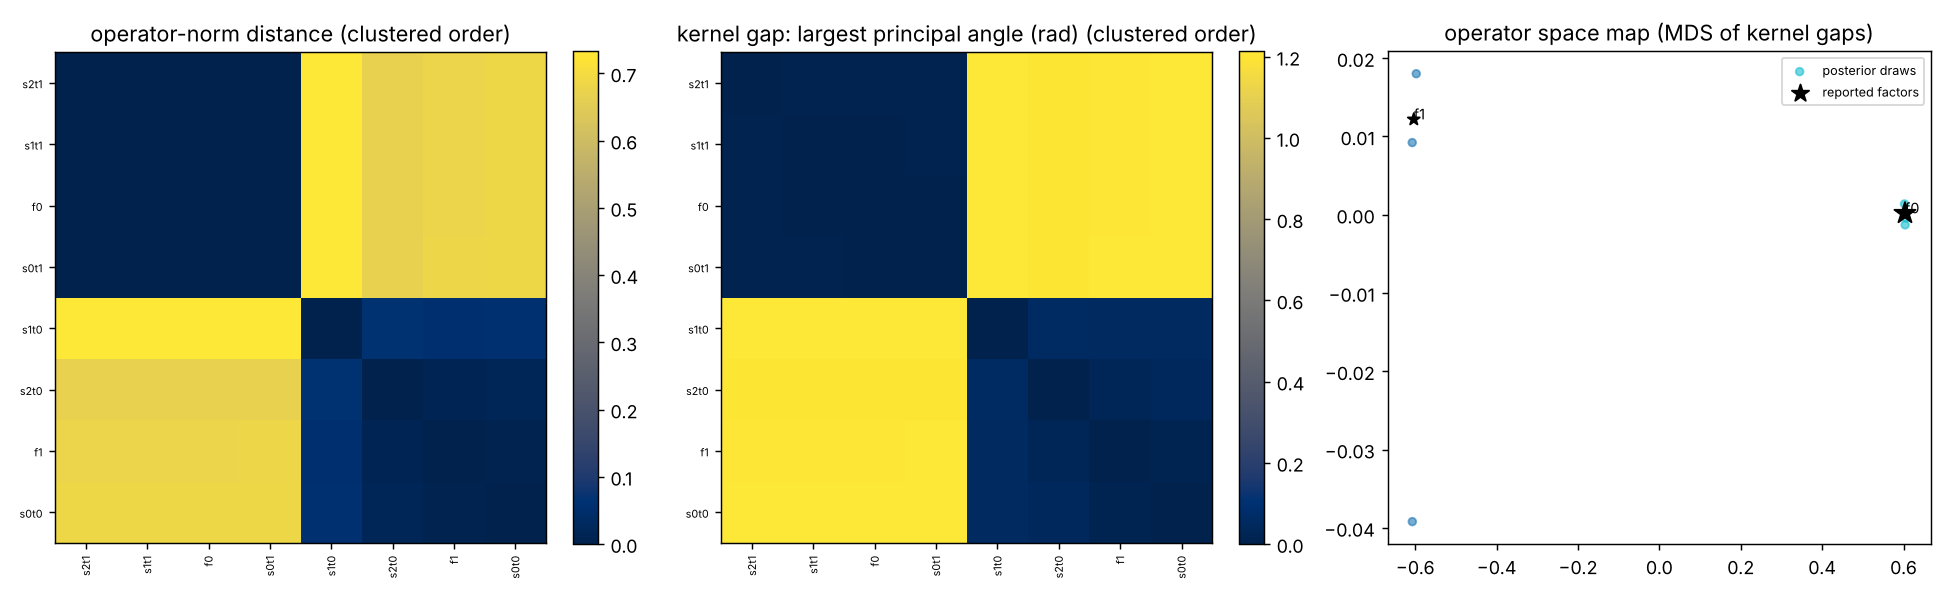
\includegraphics[width=\textwidth]{figures/rr_operator_space.png}
\caption{Left: distance between operators in operator norm (symbols normalised to unit size on the frequency box). Middle: \emph{kernel gap}, the largest principal angle (in radians) between the solution spaces of two operators; 0 means the same space, near $\pi/2$ means orthogonal. Rows and columns are the reported factors (\code{f0}, \code{f1}) and a sample of posterior draws (\code{s<sample>t<track>}), reordered by clustering so that similar operators sit together: the \textbf{dark blocks on the diagonal are clusters}, the bright off-diagonal blocks are the distance between clusters. Right: a two-dimensional map (multidimensional scaling) of the kernel gaps; stars are the reported factors (size grows with weight $W$), dots are posterior draws, coloured by track.}
\end{figure}
Reading it: two compact blobs far apart (as here: diffusion on the left, transport on the right) = two well separated factors, and the posterior draws sit on top of the reported factors, i.e.\ the posterior agrees with the report. A blob of draws that is spread out, or a cloud halfway between two stars, means that the draws disagree about the structure; two stars close together means the data hardly distinguish the factors (small $\gamma$, large amplification). The map is a 2-D drawing of distances, so only relative closeness matters, not the axis values.

\subsection{\texttt{modes\_and\_components.png}: what the factors look like as functions}
\begin{figure}[H]\centering
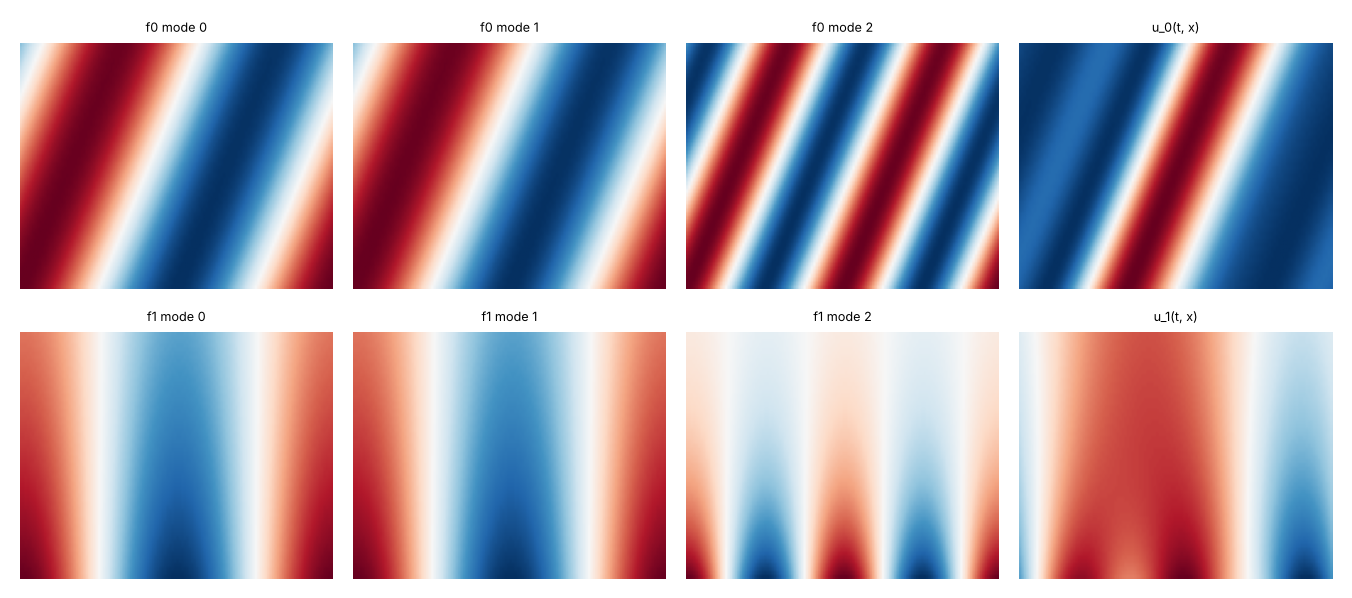
\includegraphics[width=\textwidth]{figures/rr_modes_and_components.png}
\caption{One row per factor. The first three columns are the first kernel modes of that factor, as images of $(t,x)$ with time running upward and $x$ to the right (red positive, blue negative); the last column is the \emph{component} $u_j(t,x)$ of the data attributed to that factor.}
\end{figure}
Transport modes are oblique stripes (a pattern that moves along $x$ as $t$ increases, here to the right); diffusion modes are vertical stripes that fade with time (a spatial pattern that smooths out). The component $u_j$ is the part of the observed field that factor $j$ accounts for; the sum of the components reconstructs the data (their joint relative residual, $0.015$ here, is reported in \code{fit}). If a component looks like noise or a copy of the other, the corresponding factor is not well separated.

\subsection{\texttt{distributions.png}}
Described in Figure~\ref{fig:dist}: histograms of $c_F$, $\gamma$, $\rho$ over the posterior samples.

\section{Five questions to ask of any result}
\begin{enumerate}
\item \textbf{What is the label?} Anything other than FIT-COMPATIBLE: read the note first.
\item \textbf{Are the factors separated?} $P(\text{split})$ close to 1, $\gamma$ not tiny, two distinct blobs in the operator-space map.
\item \textbf{Is each coefficient narrow and nonzero?} Look at q05--q95 of each term and at the pruned equation; discount terms that are tiny.
\item \textbf{Does the model pass the tests?} No $\log_{10}p$ below $-3$ in the note; the history shows a class that was accepted.
\item \textbf{Do the pictures look like physics?} Clean dark curves in the direction images, components that look like the data, posterior draws on top of the reported factors.
\end{enumerate}
\end{document}
